\documentclass{beamer}

%
% Common preamble for all three parts.
%

\usepackage[utf8]{inputenc}
\usepackage{lmodern}
\usepackage[english,french]{babel}
\usepackage[T1]{fontenc}
\usepackage{amsmath}
\usepackage{color}
\usepackage{minted}
\usepackage{hyperref}
\usepackage{multicol}
\usepackage{tabularx}
\usepackage{tikz}

% only inline todonotes work
\usepackage{xkeyval}
\usepackage[textsize=small]{todonotes}
\presetkeys{todonotes}{inline}{}

\usetikzlibrary{shapes,arrows,positioning,shadows}

% no nav buttons
\usenavigationsymbolstemplate{}

\newcommand{\bftt}[1]{\textbf{\texttt{#1}}}
\newcommand{\comment}[1]{{\color[HTML]{008080}\textit{\textbf{\texttt{#1}}}}}
\newcommand{\cmd}[1]{{\color[HTML]{008000}\bftt{#1}}}
\newcommand{\bs}{\char`\\}
\newcommand{\cmdbs}[1]{\cmd{\bs#1}}
\newcommand{\lcb}{\char '173}
\newcommand{\rcb}{\char '175}
\newcommand{\cmdbegin}[1]{\cmdbs{begin\lcb}\bftt{#1}\cmd{\rcb}}
\newcommand{\cmdend}[1]{\cmdbs{end\lcb}\bftt{#1}\cmd{\rcb}}

\newcommand{\wllogo}{\textbf{Overleaf}}

% c'est ici que sont chargés les sources de fichiers d'exemple
% ne pas introduire de slash final
\newcommand{\fileuri}{https://raw.github.com/jdleesmiller/latex-course/master/fr}

\newcommand{\wlserver}{https://www.overleaf.com}
\newcommand{\wlnewdoc}[1]{\wlserver/docs?snip\_uri=\fileuri/#1\&splash=none}

\def\tikzname{Ti\emph{k}Z}

% de http://tex.stackexchange.com/questions/5226/keyboard-font-for-latex
\newcommand*\keystroke[1]{%
  \tikz[baseline=(key.base)]
    \node[%
      draw,
      fill=white,
      drop shadow={shadow xshift=0.25ex,shadow yshift=-0.25ex,fill=black,opacity=0.75},
      rectangle,
      rounded corners=2pt,
      inner sep=1pt,
      line width=0.5pt,
      font=\scriptsize\sffamily
    ](key) {#1\strut}
  ;
}
\newcommand{\keystrokebftt}[1]{\keystroke{\bftt{#1}}}

% volé de minted.dtx
\newenvironment{exampletwoup}
  {\VerbatimEnvironment
   \begin{VerbatimOut}{example.out}}
  {\end{VerbatimOut}
   \setlength{\parindent}{0pt}
   \fbox{\begin{tabular}{l|l}
   \begin{minipage}{0.55\linewidth}
     \inputminted[fontsize=\small,resetmargins]{latex}{example.out}
   \end{minipage} &
   \begin{minipage}{0.35\linewidth}
     \input{example.out}
   \end{minipage}
   \end{tabular}}}

\newenvironment{exampletwouptiny}
  {\VerbatimEnvironment
   \begin{VerbatimOut}{example.out}}
  {\end{VerbatimOut}
   \setlength{\parindent}{0pt}
   \fbox{\begin{tabular}{l|l}
   \begin{minipage}{0.55\linewidth}
     \inputminted[fontsize=\scriptsize,resetmargins]{latex}{example.out}
   \end{minipage} &
   \begin{minipage}{0.35\linewidth}
     \setlength{\parskip}{6pt plus 1pt minus 1pt}%
     \raggedright\scriptsize\input{example.out}
   \end{minipage}
   \end{tabular}}}

\newenvironment{exampletwouptinynoframe}
  {\VerbatimEnvironment
   \begin{VerbatimOut}{example.out}}
  {\end{VerbatimOut}
   \setlength{\parindent}{0pt}
   \begin{tabular}{l|l}
   \begin{minipage}{0.55\linewidth}
     \inputminted[fontsize=\scriptsize,resetmargins]{latex}{example.out}
   \end{minipage} &
   \begin{minipage}{0.35\linewidth}
     \setlength{\parskip}{6pt plus 1pt minus 1pt}%
     \raggedright\scriptsize\input{example.out}
   \end{minipage}
   \end{tabular}}

\title{Une introduction interactive à \LaTeX}
\author{Dr John D. Lees-Miller\\Traduction : Yannis Haralambous (IMT Atlantique)}
\titlegraphic{%

\includegraphics[height=36pt]{overleaf}\\[1em]

\includegraphics[height=24pt]{UoB-logo}
}


\subtitle{Partie 3 : au-delà des articles --- présentations \& plus}

\newcommand{\alice}[1]{\todo[color=green!40]{#1}}
\newcommand{\bob}[1]{\todo[color=purple!40]{#1}}

\begin{document}

%%%%%%%%%%%%%%%%%%%%%%%%%%%%%%%%%%%%%%%%%%%%%%%%%%%%%%%%%%%%%%%%%%%%%%%%%%%%%%%
%%%%%%%%%%%%%%%%%%%%%%%%%%%%%%%%%%%%%%%%%%%%%%%%%%%%%%%%%%%%%%%%%%%%%%%%%%%%%%%
%%%%%%%%%%%%%%%%%%%%%%%%%%%%%%%%%%%%%%%%%%%%%%%%%%%%%%%%%%%%%%%%%%%%%%%%%%%%%%%
\begin{frame}
\titlepage
\end{frame}

%%%%%%%%%%%%%%%%%%%%%%%%%%%%%%%%%%%%%%%%%%%%%%%%%%%%%%%%%%%%%%%%%%%%%%%%%%%%%%%
%%%%%%%%%%%%%%%%%%%%%%%%%%%%%%%%%%%%%%%%%%%%%%%%%%%%%%%%%%%%%%%%%%%%%%%%%%%%%%%
%%%%%%%%%%%%%%%%%%%%%%%%%%%%%%%%%%%%%%%%%%%%%%%%%%%%%%%%%%%%%%%%%%%%%%%%%%%%%%%
%\begin{frame}{Setup}
%\begin{itemize}
%\item Go to this URL in Google Chrome (\emph{not} Internet Explorer) to open
%these slides on your computer:
%\vskip 2em
%\begin{center}
%\fbox{\url{http://bit.ly/12WWWqj}}
%\end{center}
%\vskip 2em
%\item Here are the slides from the previous tutorial, for reference:
%\begin{center}
%\vskip 1em
%\fbox{\href{https://dl.dropboxusercontent.com/u/31383671/site/latex_course_v2/part1.pdf}{Part 1: The Basics}}
%\vskip 1em
%\fbox{\href{https://dl.dropboxusercontent.com/u/31383671/site/latex_course_v2/part2.pdf}{Part 2: Structured Documents \& More}}
%\end{center}
%\end{itemize}
%\end{frame}

%%%%%%%%%%%%%%%%%%%%%%%%%%%%%%%%%%%%%%%%%%%%%%%%%%%%%%%%%%%%%%%%%%%%%%%%%%%%%%%
%%%%%%%%%%%%%%%%%%%%%%%%%%%%%%%%%%%%%%%%%%%%%%%%%%%%%%%%%%%%%%%%%%%%%%%%%%%%%%%
%%%%%%%%%%%%%%%%%%%%%%%%%%%%%%%%%%%%%%%%%%%%%%%%%%%%%%%%%%%%%%%%%%%%%%%%%%%%%%%
\section{Récapitulatif de \LaTeX{}}

%%%%%%%%%%%%%%%%%%%%%%%%%%%%%%%%%%%%%%%%%%%%%%%%%%%%%%%%%%%%%%%%%%%%%%%%%%%%%%%
%%%%%%%%%%%%%%%%%%%%%%%%%%%%%%%%%%%%%%%%%%%%%%%%%%%%%%%%%%%%%%%%%%%%%%%%%%%%%%%
%%%%%%%%%%%%%%%%%%%%%%%%%%%%%%%%%%%%%%%%%%%%%%%%%%%%%%%%%%%%%%%%%%%%%%%%%%%%%%%
\begin{frame}[fragile]{\insertsection}
\begin{itemize}
\item Vous écrivez votre document en \texttt{texte brut} parsemé de \cmd{commandes} qui décrivent sa structure et son contenu.
\item Le programme \texttt{latex} traite votre texte et vos commandes et produit un document magnifiquement présenté.
\end{itemize}
\vskip 2ex
\begin{center}
\begin{minted}[frame=single]{latex}
La plume est plus \emph{forte} que l'épée.
\end{minted}
\vskip 2ex
\tikz\node[single arrow,fill=gray,font=\ttfamily\bfseries,%
  rotate=270,xshift=-1em]{latex};
\vskip 2ex
\fbox{La plume est plus \emph{forte} que l'épée.}
\end{center}
\end{frame}

%%%%%%%%%%%%%%%%%%%%%%%%%%%%%%%%%%%%%%%%%%%%%%%%%%%%%%%%%%%%%%%%%%%%%%%%%%%%%%%
%%%%%%%%%%%%%%%%%%%%%%%%%%%%%%%%%%%%%%%%%%%%%%%%%%%%%%%%%%%%%%%%%%%%%%%%%%%%%%%
%%%%%%%%%%%%%%%%%%%%%%%%%%%%%%%%%%%%%%%%%%%%%%%%%%%%%%%%%%%%%%%%%%%%%%%%%%%%%%%
\begin{frame}[fragile]{\insertsection: commandes \& arguments}
\begin{itemize}
\item Une commande commence par un \emph{antislash} \keystrokebftt{\bs}.
\item Certaines commandes prennent un \emph{argument} entre accolades \keystrokebftt{\{}
\keystrokebftt{\}}.
\item Certaines commandes prennent également des \emph{arguments optionnels} entre crochets \keystrokebftt{[} \keystrokebftt{]}.
\vskip 2ex
\begin{exampletwouptiny}

\includegraphics[
  width=0.5\textwidth]{gerbil}


\includegraphics[
  width=0.3\textwidth,
  angle=270]{gerbil}
\end{exampletwouptiny}
\end{itemize}

\tiny{Droits d'auteur de l'image: \href{https://pixabay.com/en/animal-apple-attractive-beautiful-1239390/}{CC0}}
\end{frame}

%%%%%%%%%%%%%%%%%%%%%%%%%%%%%%%%%%%%%%%%%%%%%%%%%%%%%%%%%%%%%%%%%%%%%%%%%%%%%%%
%%%%%%%%%%%%%%%%%%%%%%%%%%%%%%%%%%%%%%%%%%%%%%%%%%%%%%%%%%%%%%%%%%%%%%%%%%%%%%%
%%%%%%%%%%%%%%%%%%%%%%%%%%%%%%%%%%%%%%%%%%%%%%%%%%%%%%%%%%%%%%%%%%%%%%%%%%%%%%%
\begin{frame}[fragile]{\insertsection: environnements}
\begin{itemize}
\item Les commandes \cmdbs{begin} et \cmdbs{end} sont utilisés pour créer une grande variété d'environnements --- contextes.

\item Les environnements \bftt{itemize} et \bftt{enumerate} produisent des listes.
\vskip 2ex
\begin{exampletwouptiny}
\begin{itemize} % pour avoir des puces
\item Biscuits
\item Thé
\end{itemize}

\begin{enumerate} % énumération
\item Biscuits
\item Thé
\end{enumerate}
\end{exampletwouptiny}

\end{itemize}
\end{frame}

%%%%%%%%%%%%%%%%%%%%%%%%%%%%%%%%%%%%%%%%%%%%%%%%%%%%%%%%%%%%%%%%%%%%%%%%%%%%%%%
%%%%%%%%%%%%%%%%%%%%%%%%%%%%%%%%%%%%%%%%%%%%%%%%%%%%%%%%%%%%%%%%%%%%%%%%%%%%%%%
%%%%%%%%%%%%%%%%%%%%%%%%%%%%%%%%%%%%%%%%%%%%%%%%%%%%%%%%%%%%%%%%%%%%%%%%%%%%%%%
\begin{frame}[fragile]{\insertsection: mathematiques}
\begin{itemize}
\item L'environnement \bftt{equation} produit des équations numérotées.
\begin{exampletwouptiny}
\begin{equation}
  \sum_{k=1}^{n} \frac{1}{2^k}
\end{equation}
\end{exampletwouptiny}
\vskip 2ex

\item Utilisez des signes de dollar \keystrokebftt{\$} pour indiquer les mathématiques dans le texte courant.\\[1ex]
\begin{exampletwouptiny}
% pas très bon :
Soient a et b des entiers positifs
distincts, et soit c = a - b + 1.

% bien mieux :
Soient $a$ et $b$ des entier positifs
distincts, et soit $c = a - b + 1$.
\end{exampletwouptiny}
\vskip 2ex
\item Toujours utiliser les signes de dollar par paires --- un pour commencer l'expression mathématiques, un autre pour la finir.
\vskip 1em
{\scriptsize En fait, on aurait pu aussi écrire \cmdbegin{math}\bftt{...}\cmdend{math} au lieu de \bftt{\$...\$}.}
\end{itemize}
\end{frame}

%%%%%%%%%%%%%%%%%%%%%%%%%%%%%%%%%%%%%%%%%%%%%%%%%%%%%%%%%%%%%%%%%%%%%%%%%%%%%%%
%%%%%%%%%%%%%%%%%%%%%%%%%%%%%%%%%%%%%%%%%%%%%%%%%%%%%%%%%%%%%%%%%%%%%%%%%%%%%%%
%%%%%%%%%%%%%%%%%%%%%%%%%%%%%%%%%%%%%%%%%%%%%%%%%%%%%%%%%%%%%%%%%%%%%%%%%%%%%%%
\begin{frame}[fragile]{\insertsection: structure de document}
\begin{itemize}{\small
\item Commencer par \cmdbs{documentclass} : quel type de document ?
\item Placer les metadonnées (\cmdbs{title} et \cmdbs{author}) et les packages dans le préambule.
\item Placer le contenu entre \cmdbegin{document} et \cmdend{document}.
\item La commande \cmdbs{maketitle} crée le titre ; les commandes \cmdbs{section} créent des sections numérotées.
}\end{itemize}
\begin{minipage}{0.55\linewidth}
\inputminted[fontsize=\scriptsize,frame=single,resetmargins]{latex}%
  {recap-structure.tex}
\end{minipage}
\begin{minipage}{0.35\linewidth}
% trim: l b r t

\includegraphics[width=\textwidth,clip,trim=1.5in 7in 3in 2in]{recap-structure.pdf}
\end{minipage}
\end{frame}

%%%%%%%%%%%%%%%%%%%%%%%%%%%%%%%%%%%%%%%%%%%%%%%%%%%%%%%%%%%%%%%%%%%%%%%%%%%%%%%
%%%%%%%%%%%%%%%%%%%%%%%%%%%%%%%%%%%%%%%%%%%%%%%%%%%%%%%%%%%%%%%%%%%%%%%%%%%%%%%
%%%%%%%%%%%%%%%%%%%%%%%%%%%%%%%%%%%%%%%%%%%%%%%%%%%%%%%%%%%%%%%%%%%%%%%%%%%%%%%
\begin{frame}[fragile]{\insertsection: exercice}

\begin{enumerate}
\item Voici le texte d'un court article\footnote{Basé sur \url{http://www.cgd.ucar.edu/cms/agu/scientific_talk.html}} :
\begin{center}
\fbox{\href{\wlnewdoc{recap-exercise.tex}}{%
Cliquez ici pour ouvrir l'exercice dans \wllogo{}}}
\end{center}
\vskip 2ex
\item Ajoutez des commandes \LaTeX{} au texte pour qu'il ressemble à ceci :
\begin{center}
\fbox{\href{\fileuri/recap-exercise-solution.pdf}, \emph{protégez}-le avec un antislash (\cmdbs{\%}).
\item Pour composer une équation, utilisez \cmdbs{frac} pour les fractions et \cmdbs{left(} et \cmdbs{right)} pour les parenthèses.
\end{itemize}
\end{block}
\end{frame}

%%%%%%%%%%%%%%%%%%%%%%%%%%%%%%%%%%%%%%%%%%%%%%%%%%%%%%%%%%%%%%%%%%%%%%%%%%%%%%%
%%%%%%%%%%%%%%%%%%%%%%%%%%%%%%%%%%%%%%%%%%%%%%%%%%%%%%%%%%%%%%%%%%%%%%%%%%%%%%%
%%%%%%%%%%%%%%%%%%%%%%%%%%%%%%%%%%%%%%%%%%%%%%%%%%%%%%%%%%%%%%%%%%%%%%%%%%%%%%%
\section{Présentations avec \protect\bftt{beamer}}

%%%%%%%%%%%%%%%%%%%%%%%%%%%%%%%%%%%%%%%%%%%%%%%%%%%%%%%%%%%%%%%%%%%%%%%%%%%%%%%
%%%%%%%%%%%%%%%%%%%%%%%%%%%%%%%%%%%%%%%%%%%%%%%%%%%%%%%%%%%%%%%%%%%%%%%%%%%%%%%
%%%%%%%%%%%%%%%%%%%%%%%%%%%%%%%%%%%%%%%%%%%%%%%%%%%%%%%%%%%%%%%%%%%%%%%%%%%%%%%
\begin{frame}[fragile]{\insertsection}
\begin{itemize}
\item Beamer est un package de création de présentations (comme celle-ci !) sous
\LaTeX{}.
\item On utilisera la classe de document \bftt{beamer}.
\item Et l'environnement \bftt{frame} pour créer des transparents.
\end{itemize}
\begin{minipage}{0.55\linewidth}
\inputminted[fontsize=\scriptsize,frame=single,resetmargins]{latex}%
  {beamer-minimal.tex}
\end{minipage}
\begin{minipage}{0.35\linewidth}
% trim: l b r t

\includegraphics[width=\textwidth,clip,trim=1in 1in 1in 1in]{beamer-minimal.pdf}
\end{minipage}
\end{frame}

%%%%%%%%%%%%%%%%%%%%%%%%%%%%%%%%%%%%%%%%%%%%%%%%%%%%%%%%%%%%%%%%%%%%%%%%%%%%%%%
%%%%%%%%%%%%%%%%%%%%%%%%%%%%%%%%%%%%%%%%%%%%%%%%%%%%%%%%%%%%%%%%%%%%%%%%%%%%%%%
%%%%%%%%%%%%%%%%%%%%%%%%%%%%%%%%%%%%%%%%%%%%%%%%%%%%%%%%%%%%%%%%%%%%%%%%%%%%%%%
\begin{frame}[fragile]{\insertsection: pour bien suivre}

\begin{itemize}
\item Pendant que nous parcourons les transparents suivants, essayez les exemples en les tapant dans l'exemple de document dans \wllogo.
\end{itemize}
\vskip 2ex
\begin{center}
\fbox{\href{\wlnewdoc{beamer-minimal.tex}}{%
Cliquez ici pour ouvrir l'exemple de document dans \wllogo{}}}
\end{center}
\end{frame}

%%%%%%%%%%%%%%%%%%%%%%%%%%%%%%%%%%%%%%%%%%%%%%%%%%%%%%%%%%%%%%%%%%%%%%%%%%%%%%%
%%%%%%%%%%%%%%%%%%%%%%%%%%%%%%%%%%%%%%%%%%%%%%%%%%%%%%%%%%%%%%%%%%%%%%%%%%%%%%%
%%%%%%%%%%%%%%%%%%%%%%%%%%%%%%%%%%%%%%%%%%%%%%%%%%%%%%%%%%%%%%%%%%%%%%%%%%%%%%%
\begin{frame}[fragile]
\frametitle{\insertsection: transparents}
\begin{itemize}
\item Utilisez \cmdbs{frametitle} pour ajouter un titre à votre transparent.
\item Ensuite ajoutez du contenu au transparent.
\item Le source du transparent ressemble à ceci :
\vskip 2ex
\inputminted[fontsize=\scriptsize,frame=single,resetmargins]{latex}%
  {beamer-frame.tex}
\end{itemize}
\end{frame}

%%%%%%%%%%%%%%%%%%%%%%%%%%%%%%%%%%%%%%%%%%%%%%%%%%%%%%%%%%%%%%%%%%%%%%%%%%%%%%%
%%%%%%%%%%%%%%%%%%%%%%%%%%%%%%%%%%%%%%%%%%%%%%%%%%%%%%%%%%%%%%%%%%%%%%%%%%%%%%%
%%%%%%%%%%%%%%%%%%%%%%%%%%%%%%%%%%%%%%%%%%%%%%%%%%%%%%%%%%%%%%%%%%%%%%%%%%%%%%%
\begin{frame}[fragile]{\insertsection: sections}
\begin{itemize}
\item Vous pouvez utiliser des commandes \cmdbs{section} pour grouper vos transparents \bftt{frame}, et
\bftt{beamer} s'en servira pour créer une table de matières automatique.
\item Pour générer une table de matières, utilisez la commande \cmdbs{tableofcontents}. Voici celle de cette présentation. L'option \bftt{currentsection} met en évidence la section courante.
\vskip 2ex
\begin{exampletwouptiny}
\tableofcontents[currentsection]
\end{exampletwouptiny}
\end{itemize}
\end{frame}

%%%%%%%%%%%%%%%%%%%%%%%%%%%%%%%%%%%%%%%%%%%%%%%%%%%%%%%%%%%%%%%%%%%%%%%%%%%%%%%
%%%%%%%%%%%%%%%%%%%%%%%%%%%%%%%%%%%%%%%%%%%%%%%%%%%%%%%%%%%%%%%%%%%%%%%%%%%%%%%
%%%%%%%%%%%%%%%%%%%%%%%%%%%%%%%%%%%%%%%%%%%%%%%%%%%%%%%%%%%%%%%%%%%%%%%%%%%%%%%
\begin{frame}[fragile]{\insertsection: multicolonnage}
\begin{columns}
\begin{column}{0.4\textwidth}
\begin{itemize}
\item Utilisez les environnements \bftt{columns} et \bftt{column} pour diviser votre transparent en plusieurs colonnes.
\item L'argument de chaque \bftt{column} détermine sa largeur.
\item Cf. aussi le package \bftt{multicol} qui divise automatiquement votre contenu en colonnes.
\end{itemize}
\end{column}
\begin{column}{0.6\textwidth}
\begin{minted}[fontsize=\scriptsize,frame=single]{latex}
\begin{columns}
  \begin{column}{0.4\textwidth}
    \begin{itemize}
    \item Utilisez les environnements ...
    \item L'argument de chaque ...
    \item Cf. aussi le package ...
    \end{itemize}
  \end{column}
  \begin{column}{0.6\textwidth}
    % deuxième colonne
  \end{column}
\end{columns}
\end{minted}
\end{column}
\end{columns}
\end{frame}

%%%%%%%%%%%%%%%%%%%%%%%%%%%%%%%%%%%%%%%%%%%%%%%%%%%%%%%%%%%%%%%%%%%%%%%%%%%%%%%
%%%%%%%%%%%%%%%%%%%%%%%%%%%%%%%%%%%%%%%%%%%%%%%%%%%%%%%%%%%%%%%%%%%%%%%%%%%%%%%
%%%%%%%%%%%%%%%%%%%%%%%%%%%%%%%%%%%%%%%%%%%%%%%%%%%%%%%%%%%%%%%%%%%%%%%%%%%%%%%
\begin{frame}[fragile]{\insertsection: mise en évidence}
\begin{itemize}

\item Utilisez les commandes \cmdbs{emph} ou \cmdbs{alert} pour mettre en évidence :
\vskip 1ex
\begin{exampletwouptiny}
Je voudrais \emph{mettre en évidence}
le fait que ceci est un
point \alert{important}.
\end{exampletwouptiny}
\vskip 1ex

\item Spécifiez un caractère gras ou italique :
\vskip 1ex
\begin{exampletwouptiny}
Texte en \textbf{gras}.
Texte en \textit{italiques}.
\end{exampletwouptiny}
\vskip 1ex

\item Spécifiez une couleur :
\vskip 1ex
\begin{exampletwouptiny}
il s'\textcolor{red}{arrête}
et il \textcolor{green}{recommence}.
\end{exampletwouptiny}
\vskip 1ex
\item Cf. \url{http://www.math.umbc.edu/~rouben/beamer/quickstart-Z-H-25.html}
pour avoir plus de couleurs, y compris des couleurs personnalisées.
\end{itemize}
\end{frame}

%%%%%%%%%%%%%%%%%%%%%%%%%%%%%%%%%%%%%%%%%%%%%%%%%%%%%%%%%%%%%%%%%%%%%%%%%%%%%%%
%%%%%%%%%%%%%%%%%%%%%%%%%%%%%%%%%%%%%%%%%%%%%%%%%%%%%%%%%%%%%%%%%%%%%%%%%%%%%%%
%%%%%%%%%%%%%%%%%%%%%%%%%%%%%%%%%%%%%%%%%%%%%%%%%%%%%%%%%%%%%%%%%%%%%%%%%%%%%%%
\begin{frame}[fragile]{\insertsection: figures}
\begin{itemize}
\item Utilisez \cmdbs{includegraphics} du package \bftt{graphicx}.
\item L'environnement \bftt{figure} est, par défaut, centré sous \bftt{beamer}.
\vskip 2ex
\begin{exampletwouptiny}
\begin{figure}

\includegraphics[
  width=0.5\textwidth]{gerbil}
\end{figure}
\end{exampletwouptiny}
\end{itemize}

\tiny{Droits d'auteur de l'image: \href{https://pixabay.com/en/animal-apple-attractive-beautiful-1239390/}{CC0}}
\end{frame}

%%%%%%%%%%%%%%%%%%%%%%%%%%%%%%%%%%%%%%%%%%%%%%%%%%%%%%%%%%%%%%%%%%%%%%%%%%%%%%%
%%%%%%%%%%%%%%%%%%%%%%%%%%%%%%%%%%%%%%%%%%%%%%%%%%%%%%%%%%%%%%%%%%%%%%%%%%%%%%%
%%%%%%%%%%%%%%%%%%%%%%%%%%%%%%%%%%%%%%%%%%%%%%%%%%%%%%%%%%%%%%%%%%%%%%%%%%%%%%%
\begin{frame}[fragile]{\insertsection: tableaux}
\begin{itemize}
\item Les tableaux sous \LaTeX{} demandent un peu d'entraînement.
\item Utilisez l'environnement \bftt{tabular} du package \bftt{tabularx}.
\item L'argument spécifie l'alignement des colonnes --- \textbf{l} = fer à gauche, \textbf{r} = fer à droite, \textbf{r} = fer à droite.
\begin{exampletwouptiny}
\begin{tabular}{lrr}
Item   & Qté & Prix en \$ \\
Widget & 1   & 199,99  \\
Gadget & 2   & 399,99  \\
Câble  & 3   & 19,99   \\
\end{tabular}
\end{exampletwouptiny}
\item Il spécifie également les filets verticaux ; utilisez \cmdbs{hline} pour les filets horizontaux.
\begin{exampletwouptiny}
\begin{tabular}{|l|r|r|} \hline
Item   & Qté & Prix en \$ \\\hline
Widget & 1   & 199,99  \\
Gadget & 2   & 399,99  \\
Câble  & 3   & 19,99   \\\hline
\end{tabular}
\end{exampletwouptiny}
\item Utilisez une esperluette \keystrokebftt{\&} pour séparer les colonnes et un double antislash \keystrokebftt{\bs}\keystrokebftt{\bs} pour passer à la ligne (comme dans l'env.t \bftt{align*} que nous avons vu dans la première partie).
\end{itemize}
\end{frame}

%%%%%%%%%%%%%%%%%%%%%%%%%%%%%%%%%%%%%%%%%%%%%%%%%%%%%%%%%%%%%%%%%%%%%%%%%%%%%%%
%%%%%%%%%%%%%%%%%%%%%%%%%%%%%%%%%%%%%%%%%%%%%%%%%%%%%%%%%%%%%%%%%%%%%%%%%%%%%%%
%%%%%%%%%%%%%%%%%%%%%%%%%%%%%%%%%%%%%%%%%%%%%%%%%%%%%%%%%%%%%%%%%%%%%%%%%%%%%%%
\begin{frame}[fragile]{\insertsection: blocs}
\begin{itemize}
\item \mbox{Un environnement} de bloc \bftt{block} crée une boîte entourée d'un filet.
\begin{exampletwouptiny}
\begin{block}{Fait intéressant}
Ceci est important, n'est-il pas ?
\end{block}

\begin{alertblock}{Récit édifiant}
Ceci, par contre, est vraiment
important !
\end{alertblock}
\end{exampletwouptiny}

\item Son apparence exacte dépend du thème...
\end{itemize}
\end{frame}

%%%%%%%%%%%%%%%%%%%%%%%%%%%%%%%%%%%%%%%%%%%%%%%%%%%%%%%%%%%%%%%%%%%%%%%%%%%%%%%
%%%%%%%%%%%%%%%%%%%%%%%%%%%%%%%%%%%%%%%%%%%%%%%%%%%%%%%%%%%%%%%%%%%%%%%%%%%%%%%
%%%%%%%%%%%%%%%%%%%%%%%%%%%%%%%%%%%%%%%%%%%%%%%%%%%%%%%%%%%%%%%%%%%%%%%%%%%%%%%
\begin{frame}[fragile]
\frametitle{\insertsection: thèmes}
\begin{itemize}
\item Personnalisez votre présentation en utilisant des thèmes.
\item Cf. \url{http://deic.uab.es/~iblanes/beamer_gallery/index_by_theme.html}
pour une large collection de thèmes.
\end{itemize}
\begin{minipage}{0.55\linewidth}
\inputminted[fontsize=\scriptsize,frame=single,resetmargins]{latex}%
  {beamer-theme.tex}
\end{minipage}
\begin{minipage}{0.35\linewidth}
% trim: l b r t
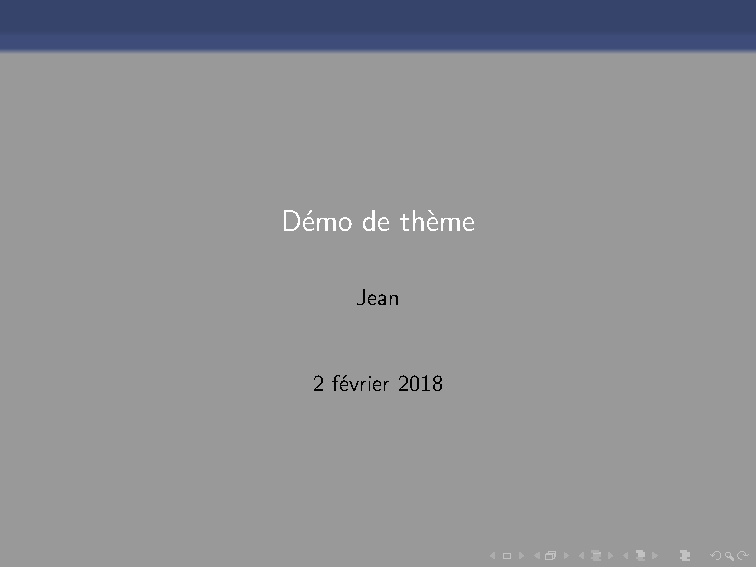
\includegraphics[width=\textwidth]{beamer-theme.pdf}
\end{minipage}
\end{frame}

%%%%%%%%%%%%%%%%%%%%%%%%%%%%%%%%%%%%%%%%%%%%%%%%%%%%%%%%%%%%%%%%%%%%%%%%%%%%%%%
%%%%%%%%%%%%%%%%%%%%%%%%%%%%%%%%%%%%%%%%%%%%%%%%%%%%%%%%%%%%%%%%%%%%%%%%%%%%%%%
%%%%%%%%%%%%%%%%%%%%%%%%%%%%%%%%%%%%%%%%%%%%%%%%%%%%%%%%%%%%%%%%%%%%%%%%%%%%%%%
\begin{frame}[fragile]{\insertsection: animations}
\begin{itemize}
\item Un environnement \bftt{frame} peut générer plusieurs transparents.
\item Utilisez la commande \cmdbs{pause} pour montrer uniquement une partie du transparent.
\vskip 2ex
\begin{exampletwouptinynoframe}
\begin{itemize}
\item Sentez-vous 
\pause \item l'anticipation ?
\end{itemize}
\end{exampletwouptinynoframe}
\vskip 2ex
\item Il y a des manières plus futées pour créer des animations sous \bftt{beamer}; cf.
aussi les commandes \cmdbs{only}, \cmdbs{alt} et \cmdbs{uncover}.
\end{itemize}
\end{frame}

%%%%%%%%%%%%%%%%%%%%%%%%%%%%%%%%%%%%%%%%%%%%%%%%%%%%%%%%%%%%%%%%%%%%%%%%%%%%%%%
%%%%%%%%%%%%%%%%%%%%%%%%%%%%%%%%%%%%%%%%%%%%%%%%%%%%%%%%%%%%%%%%%%%%%%%%%%%%%%%
%%%%%%%%%%%%%%%%%%%%%%%%%%%%%%%%%%%%%%%%%%%%%%%%%%%%%%%%%%%%%%%%%%%%%%%%%%%%%%%
\begin{frame}[fragile]{\insertsection: exercice}

Créer de nouveau l'excellente \og Présentation PowerPoint de Gettysburg\fg{} sous \bftt{beamer}\footnote{\url{http://norvig.com/Gettysburg}}.

\begin{enumerate}
\item Ouvrez l'exercice dans \wllogo{}:
\begin{center}
\fbox{\href{\wlnewdoc{beamer-exercise.tex}}{%
Cliquez ici pour ouvrir l'exercice dans \wllogo{}}}
\end{center}
\vskip 2ex
\item Téléchargez cette image sur votre machine et envoyez-la à \wllogo{} par le biais du menu de fichier.
\begin{center}
\fbox{\href{\fileuri/gettysburg_graph.png?dl=1}{Cliquez ici pour télécharger l'image}}
\end{center}
\vskip 2ex
\item Ajoutez des commandes \LaTeX{} au texte pour rendre votre document semblable à celui-ci:
\begin{center}
\fbox{\href{\fileuri/beamer-exercise-solution.pdf}{%
Cliquez ici pour ouvrir le modèle de document}}
\end{center}
\end{enumerate}
\end{frame}

%%%%%%%%%%%%%%%%%%%%%%%%%%%%%%%%%%%%%%%%%%%%%%%%%%%%%%%%%%%%%%%%%%%%%%%%%%%%%%%
%%%%%%%%%%%%%%%%%%%%%%%%%%%%%%%%%%%%%%%%%%%%%%%%%%%%%%%%%%%%%%%%%%%%%%%%%%%%%%%
%%%%%%%%%%%%%%%%%%%%%%%%%%%%%%%%%%%%%%%%%%%%%%%%%%%%%%%%%%%%%%%%%%%%%%%%%%%%%%%
\section{Dessiner des schémas avec \protect\tikzname}

%%%%%%%%%%%%%%%%%%%%%%%%%%%%%%%%%%%%%%%%%%%%%%%%%%%%%%%%%%%%%%%%%%%%%%%%%%%%%%%
%%%%%%%%%%%%%%%%%%%%%%%%%%%%%%%%%%%%%%%%%%%%%%%%%%%%%%%%%%%%%%%%%%%%%%%%%%%%%%%
%%%%%%%%%%%%%%%%%%%%%%%%%%%%%%%%%%%%%%%%%%%%%%%%%%%%%%%%%%%%%%%%%%%%%%%%%%%%%%%
\begin{frame}[fragile]{\insertsection}
\begin{itemize}
\item \tikzname{} est un package permettant de dessiner des schémas sous \LaTeX.
\item Il définit un puissant langage de dessin, à l'interieur de \LaTeX{}. Des programmes très courts peuvent vous surprendre par la complexité de leurs sorties.
\begin{figure}
\href{http://www.texample.net/tikz/examples/rotated-triangle/}{%
  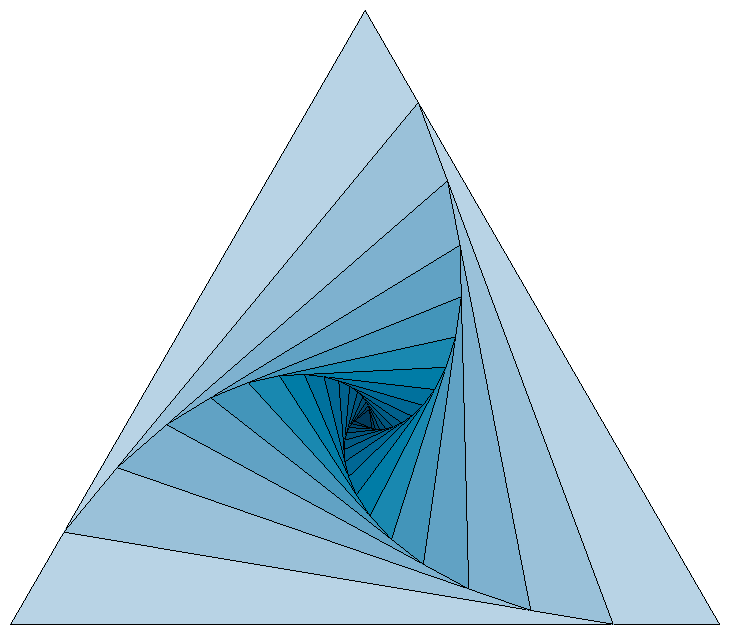
\includegraphics[width=0.35\textwidth]{rotated-triangle}}
\end{figure}
\item Nous commencerons par des choses simples. Tracez une ligne sous \tikzname :
\vskip 1ex
\begin{exampletwouptiny}
\begin{tikzpicture}
\draw (0,0) -- (1,1); % une ligne
\end{tikzpicture}
\end{exampletwouptiny}
\end{itemize}
\end{frame}

%%%%%%%%%%%%%%%%%%%%%%%%%%%%%%%%%%%%%%%%%%%%%%%%%%%%%%%%%%%%%%%%%%%%%%%%%%%%%%%
%%%%%%%%%%%%%%%%%%%%%%%%%%%%%%%%%%%%%%%%%%%%%%%%%%%%%%%%%%%%%%%%%%%%%%%%%%%%%%%
%%%%%%%%%%%%%%%%%%%%%%%%%%%%%%%%%%%%%%%%%%%%%%%%%%%%%%%%%%%%%%%%%%%%%%%%%%%%%%%
\begin{frame}[fragile]{\insertsection: coordonnées}
\begin{itemize}
\item Les coordonnées par défaut sont en centimètres dans l'ordre usuel : 
\begin{figure}
\begin{tikzpicture}[scale=0.5]
\draw[help lines] (0,0) grid (3,3);
\node[below left] at (0,0) {$(0,0)$};
\node[below right] at (3,0) {$(3,0)$};
\node[above right] at (3,3) {$(3,3)$};
\node[above left] at (0,3) {$(0,3)$};
\end{tikzpicture}
\end{figure}
\item Il peut être utile de tracer une grille quand vous travaillez avec \tikzname :
\vskip 1ex
\begin{exampletwouptiny}
\begin{tikzpicture}
\draw[help lines] (0,0) grid (3,3);
\end{tikzpicture}
\end{exampletwouptiny}
\end{itemize}
\end{frame}

%%%%%%%%%%%%%%%%%%%%%%%%%%%%%%%%%%%%%%%%%%%%%%%%%%%%%%%%%%%%%%%%%%%%%%%%%%%%%%%
%%%%%%%%%%%%%%%%%%%%%%%%%%%%%%%%%%%%%%%%%%%%%%%%%%%%%%%%%%%%%%%%%%%%%%%%%%%%%%%
%%%%%%%%%%%%%%%%%%%%%%%%%%%%%%%%%%%%%%%%%%%%%%%%%%%%%%%%%%%%%%%%%%%%%%%%%%%%%%%
\begin{frame}[fragile]{\insertsection: lignes}
\begin{itemize}
\item Les têtes de flèche et les styles de ligne sont spécifiés en tant qu'options de la commande \cmdbs{draw}.
\item Terminez chaque commande \cmdbs{draw} par un point-virgule \keystrokebftt{;}.
\vskip 1ex
\begin{exampletwouptiny}
\begin{tikzpicture}
\draw[help lines] (0,0) grid (3,3);
\draw[->] (0,0) -- (1,1);
\draw[<->, thick] (2,1) -- (1,2);
\draw[<-, thick, dashed] (2,2)--(3,3);
\end{tikzpicture}
\end{exampletwouptiny}
\end{itemize}
\end{frame}

%%%%%%%%%%%%%%%%%%%%%%%%%%%%%%%%%%%%%%%%%%%%%%%%%%%%%%%%%%%%%%%%%%%%%%%%%%%%%%%
%%%%%%%%%%%%%%%%%%%%%%%%%%%%%%%%%%%%%%%%%%%%%%%%%%%%%%%%%%%%%%%%%%%%%%%%%%%%%%%
%%%%%%%%%%%%%%%%%%%%%%%%%%%%%%%%%%%%%%%%%%%%%%%%%%%%%%%%%%%%%%%%%%%%%%%%%%%%%%%
\begin{frame}[fragile]{\insertsection: chemins}
\begin{itemize}
\item Vous pouvez spécifier plusieurs points pour former un chemin.
\item Les têtes de flèches n'apparaîtront qu'à l'extrémité du chemin.
\vskip 1ex
\begin{exampletwouptiny}
\begin{tikzpicture}
\draw[help lines] (0,0) grid (3,3);
% axes :
\draw[<->, thick] (0,3)--(0,0)--(3,0);
% diamant :
\draw (1.5,0.5) -- (2.5,1.5) -- 
      (1.5,2.5) -- (0.5,1.5) --
      cycle; % pour fermer le chemin
\end{tikzpicture}
\end{exampletwouptiny}
\end{itemize}
\end{frame}

%%%%%%%%%%%%%%%%%%%%%%%%%%%%%%%%%%%%%%%%%%%%%%%%%%%%%%%%%%%%%%%%%%%%%%%%%%%%%%%
%%%%%%%%%%%%%%%%%%%%%%%%%%%%%%%%%%%%%%%%%%%%%%%%%%%%%%%%%%%%%%%%%%%%%%%%%%%%%%%
%%%%%%%%%%%%%%%%%%%%%%%%%%%%%%%%%%%%%%%%%%%%%%%%%%%%%%%%%%%%%%%%%%%%%%%%%%%%%%%
\begin{frame}[fragile]{\insertsection: couleurs}
\begin{itemize}
\item Les couleurs sont également spécifiées en tant qu'options de la commande \cmdbs{draw}.
\vskip 1ex
\begin{exampletwouptiny}
\begin{tikzpicture}
\draw[help lines] (0,0) grid (3,3);
% axes
\draw[<->, thick, red]
  (0,3)--(0,0)--(3,0); 
% diamant
\draw[thick, blue, fill=yellow]
  (1.5,0.5) -- (2.5,1.5) -- 
  (1.5,2.5) -- (0.5,1.5) --
  cycle;
\end{tikzpicture}
\end{exampletwouptiny}
\end{itemize}
\end{frame}

%%%%%%%%%%%%%%%%%%%%%%%%%%%%%%%%%%%%%%%%%%%%%%%%%%%%%%%%%%%%%%%%%%%%%%%%%%%%%%%
%%%%%%%%%%%%%%%%%%%%%%%%%%%%%%%%%%%%%%%%%%%%%%%%%%%%%%%%%%%%%%%%%%%%%%%%%%%%%%%
%%%%%%%%%%%%%%%%%%%%%%%%%%%%%%%%%%%%%%%%%%%%%%%%%%%%%%%%%%%%%%%%%%%%%%%%%%%%%%%
\begin{frame}[fragile]{\insertsection: formes}
\begin{itemize}
\item \tikzname{} a des commandes prédéfinies pour les formes simples.
\vskip 1ex
\begin{exampletwouptiny}
\begin{tikzpicture}
\draw[help lines] (0,0) grid (3,3);
\draw (1.5,2.0) circle (0.5);
\draw (0.5,0.5) rectangle (2.5,1.5);
\end{tikzpicture}
\end{exampletwouptiny}
\end{itemize}
\end{frame}

%%%%%%%%%%%%%%%%%%%%%%%%%%%%%%%%%%%%%%%%%%%%%%%%%%%%%%%%%%%%%%%%%%%%%%%%%%%%%%%
%%%%%%%%%%%%%%%%%%%%%%%%%%%%%%%%%%%%%%%%%%%%%%%%%%%%%%%%%%%%%%%%%%%%%%%%%%%%%%%
%%%%%%%%%%%%%%%%%%%%%%%%%%%%%%%%%%%%%%%%%%%%%%%%%%%%%%%%%%%%%%%%%%%%%%%%%%%%%%%
\begin{frame}[fragile]{\insertsection: n{\oe}uds \& labels}
\begin{itemize}
\item Utilisez les n{\oe}uds \texttt{node} pour placer du texte (ou des mathématiques) dans les schémas \tikzname{}.
\item Vous pouvez aussi utiliser les n{\oe}uds en tant que coordonnées --- ce qui peut être utile pour les diagrammes.
\vskip 1ex
\begin{exampletwouptiny}
\begin{tikzpicture}
\draw[help lines] (0,0) grid (3,3);
\node (h) at (0,0) {H};
\node (x) at (1.5,1.5) {$\xi$};
\node (t) at (3,0) {T};
\draw[->] (x) -- (h);
\draw[->] (x) -- (t);
\end{tikzpicture}
\end{exampletwouptiny}
\end{itemize}
\end{frame}

%%%%%%%%%%%%%%%%%%%%%%%%%%%%%%%%%%%%%%%%%%%%%%%%%%%%%%%%%%%%%%%%%%%%%%%%%%%%%%%
%%%%%%%%%%%%%%%%%%%%%%%%%%%%%%%%%%%%%%%%%%%%%%%%%%%%%%%%%%%%%%%%%%%%%%%%%%%%%%%
%%%%%%%%%%%%%%%%%%%%%%%%%%%%%%%%%%%%%%%%%%%%%%%%%%%%%%%%%%%%%%%%%%%%%%%%%%%%%%%
\begin{frame}[fragile]{\insertsection: fonctions}
\begin{itemize}
\item Vous pouvez même tracer certaines fonctions simples.
\vskip 1ex
\begin{exampletwouptiny}
\begin{tikzpicture}[scale=0.5]
% axe des y
\draw[<->, thick] (0,2) -- (0,-2);
% axe des x
\draw[ ->, thick] (0,0) -- (7, 0); 
% courbes
\draw[cyan,domain=0:2*pi]
  plot (\x, {sin(\x r)});
\draw[magenta,domain=0:2*pi]
  plot (\x, {cos(\x r)});
\end{tikzpicture}
\end{exampletwouptiny}
\end{itemize}
\end{frame}

%%%%%%%%%%%%%%%%%%%%%%%%%%%%%%%%%%%%%%%%%%%%%%%%%%%%%%%%%%%%%%%%%%%%%%%%%%%%%%%
%%%%%%%%%%%%%%%%%%%%%%%%%%%%%%%%%%%%%%%%%%%%%%%%%%%%%%%%%%%%%%%%%%%%%%%%%%%%%%%
%%%%%%%%%%%%%%%%%%%%%%%%%%%%%%%%%%%%%%%%%%%%%%%%%%%%%%%%%%%%%%%%%%%%%%%%%%%%%%%
\begin{frame}[fragile]{\insertsection: exemples}
\begin{itemize}
\item Cf. \fbox{\href{http://texample.net/tikz/}{\TeX{}ample.net}} pour une multitude d'exemples \tikzname{} :
\end{itemize}
\begin{figure}
\href{http://texample.net/tikz/examples/escher-brick-penrose-triangle/}{%
  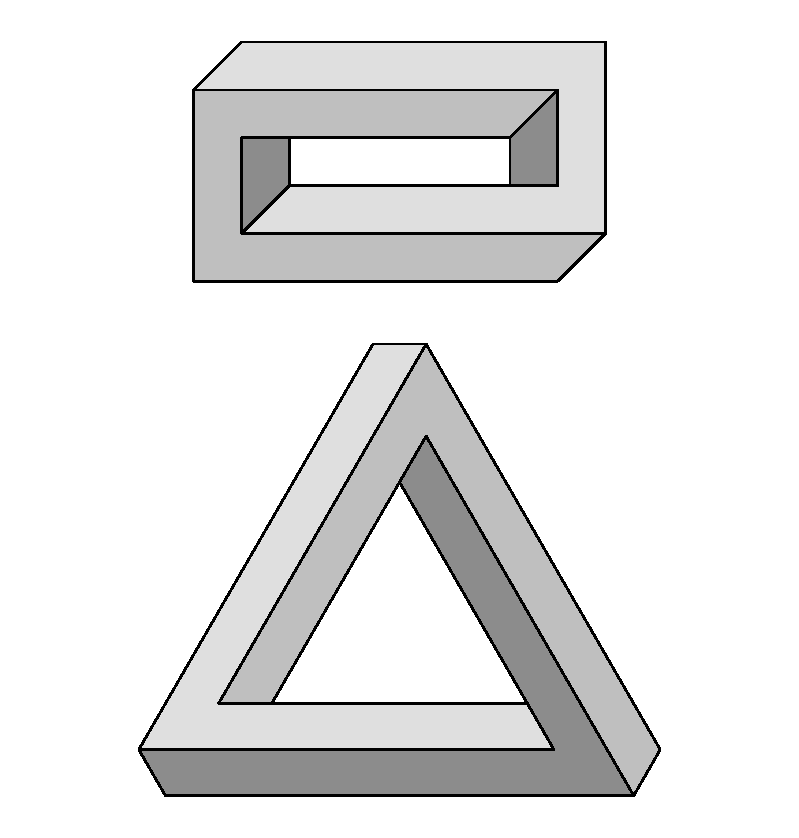
\includegraphics[width=0.3\textwidth]{escher-brick-penrose-triangle}}
\href{http://texample.net/tikz/examples/computer-science-mindmap/}{%
  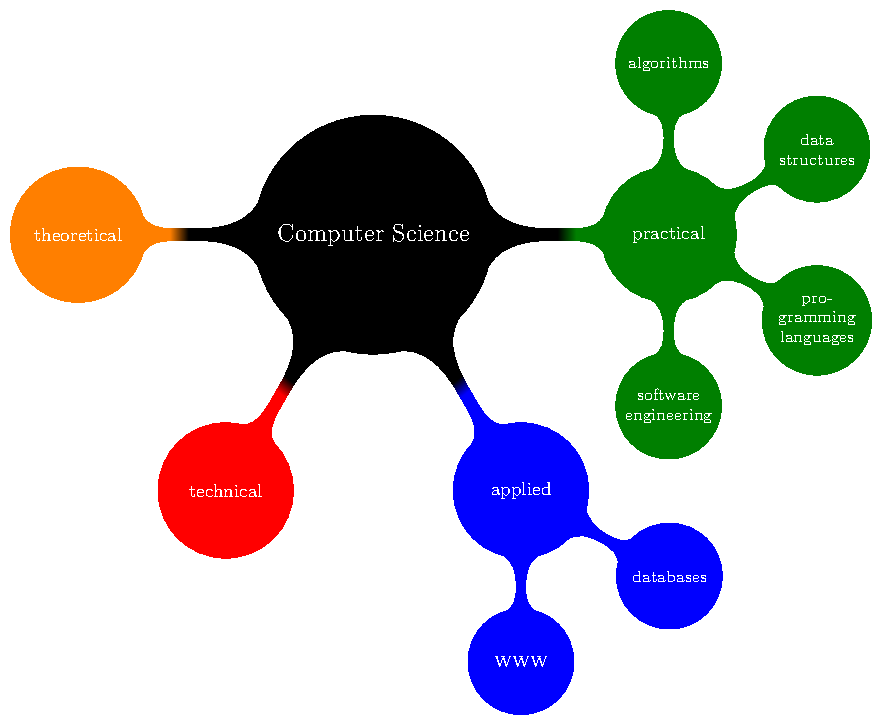
\includegraphics[width=0.3\textwidth]{computer-science-mindmap}}
\href{http://texample.net/tikz/examples/gajski-kuhn-y-chart/}{%
  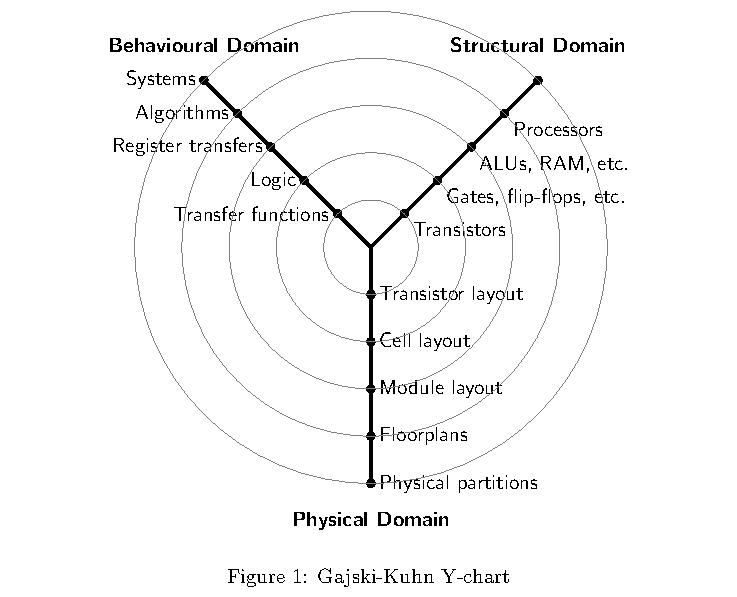
\includegraphics[width=0.3\textwidth]{gajski-kuhn-y-chart}}
\end{figure}
\end{frame}

%%%%%%%%%%%%%%%%%%%%%%%%%%%%%%%%%%%%%%%%%%%%%%%%%%%%%%%%%%%%%%%%%%%%%%%%%%%%%%%
%%%%%%%%%%%%%%%%%%%%%%%%%%%%%%%%%%%%%%%%%%%%%%%%%%%%%%%%%%%%%%%%%%%%%%%%%%%%%%%
%%%%%%%%%%%%%%%%%%%%%%%%%%%%%%%%%%%%%%%%%%%%%%%%%%%%%%%%%%%%%%%%%%%%%%%%%%%%%%%
\begin{frame}[fragile]{\insertsection: exercice}
Tracez ceci sous \tikzname\footnote{Basé sur \url{http://xkcd.com/1022}}:
\begin{figure}
\begin{tikzpicture}
\draw[help lines] (0,0) grid (6,6);
\draw[thick] (2,3) circle (0.5);
\draw[thick] (2,2.5) -- (2,1);              % body
\draw[thick] (1,1.5) -- (2,2) -- (3,1.5);   % arms
\draw[thick] (1.5, 0) -- (2,1) -- (2.5, 0); % legs
\draw[blue] (2,4) rectangle (6,6);
\draw[blue] (2.5,3.5) circle (0.1);
\draw[blue] (2.8,3.8) circle (0.15);
\node at (4,5) {So it has come to this.};
\end{tikzpicture}

\end{figure}
\end{frame}

%%%%%%%%%%%%%%%%%%%%%%%%%%%%%%%%%%%%%%%%%%%%%%%%%%%%%%%%%%%%%%%%%%%%%%%%%%%%%%%
%%%%%%%%%%%%%%%%%%%%%%%%%%%%%%%%%%%%%%%%%%%%%%%%%%%%%%%%%%%%%%%%%%%%%%%%%%%%%%%
%%%%%%%%%%%%%%%%%%%%%%%%%%%%%%%%%%%%%%%%%%%%%%%%%%%%%%%%%%%%%%%%%%%%%%%%%%%%%%%
\section{Insérer des notes avec \protect\bftt{todonotes}}

%%%%%%%%%%%%%%%%%%%%%%%%%%%%%%%%%%%%%%%%%%%%%%%%%%%%%%%%%%%%%%%%%%%%%%%%%%%%%%%
%%%%%%%%%%%%%%%%%%%%%%%%%%%%%%%%%%%%%%%%%%%%%%%%%%%%%%%%%%%%%%%%%%%%%%%%%%%%%%%
%%%%%%%%%%%%%%%%%%%%%%%%%%%%%%%%%%%%%%%%%%%%%%%%%%%%%%%%%%%%%%%%%%%%%%%%%%%%%%%
\begin{frame}[fragile]{\insertsection}
\begin{itemize}
\item La commande \cmdbs{todo} (= \og{}ce qui reste à faire\fg{}) du package \bftt{todonotes} est bien \mbox{indiquée} pour laisser des notes à vous-même et à vos collaborateurs.
\begin{exampletwouptiny}
\todo{ajouter des résultats}
\todo[color=blue!20]{corriger
la méthode}
\end{exampletwouptiny}
\vskip 2ex
\item Le tuyau du professionnel : définissez vos propres commandes avec \cmdbs{newcommand} :
\begin{minted}[fontsize=\scriptsize,frame=single]{latex}
\newcommand{\alice}[1]{\todo[color=green!40]{#1}}
\newcommand{\bob}[1]{\todo[color=purple!40]{#1}}
\end{minted}
Cela peut vous faire gagner du temps :
\begin{exampletwouptiny}
\alice{ajouter des résultats}
\bob{corriger la méthode}
\end{exampletwouptiny}
\end{itemize}
\end{frame}

%%%%%%%%%%%%%%%%%%%%%%%%%%%%%%%%%%%%%%%%%%%%%%%%%%%%%%%%%%%%%%%%%%%%%%%%%%%%%%%
%%%%%%%%%%%%%%%%%%%%%%%%%%%%%%%%%%%%%%%%%%%%%%%%%%%%%%%%%%%%%%%%%%%%%%%%%%%%%%%
%%%%%%%%%%%%%%%%%%%%%%%%%%%%%%%%%%%%%%%%%%%%%%%%%%%%%%%%%%%%%%%%%%%%%%%%%%%%%%%
\begin{frame}[fragile]{\insertsection}
\begin{columns}
  \begin{column}{0.4\textwidth}
    \begin{itemize}
    \item Beamer n'accepte que les notes internes, mais dans les documents standard vous pouvez aussi utiliser des notes marginales.
    \item Il existe aussi une commande \cmdbs{listoftodos} bien utile.
    \end{itemize}
  \end{column}
  \begin{column}{0.6\textwidth}
    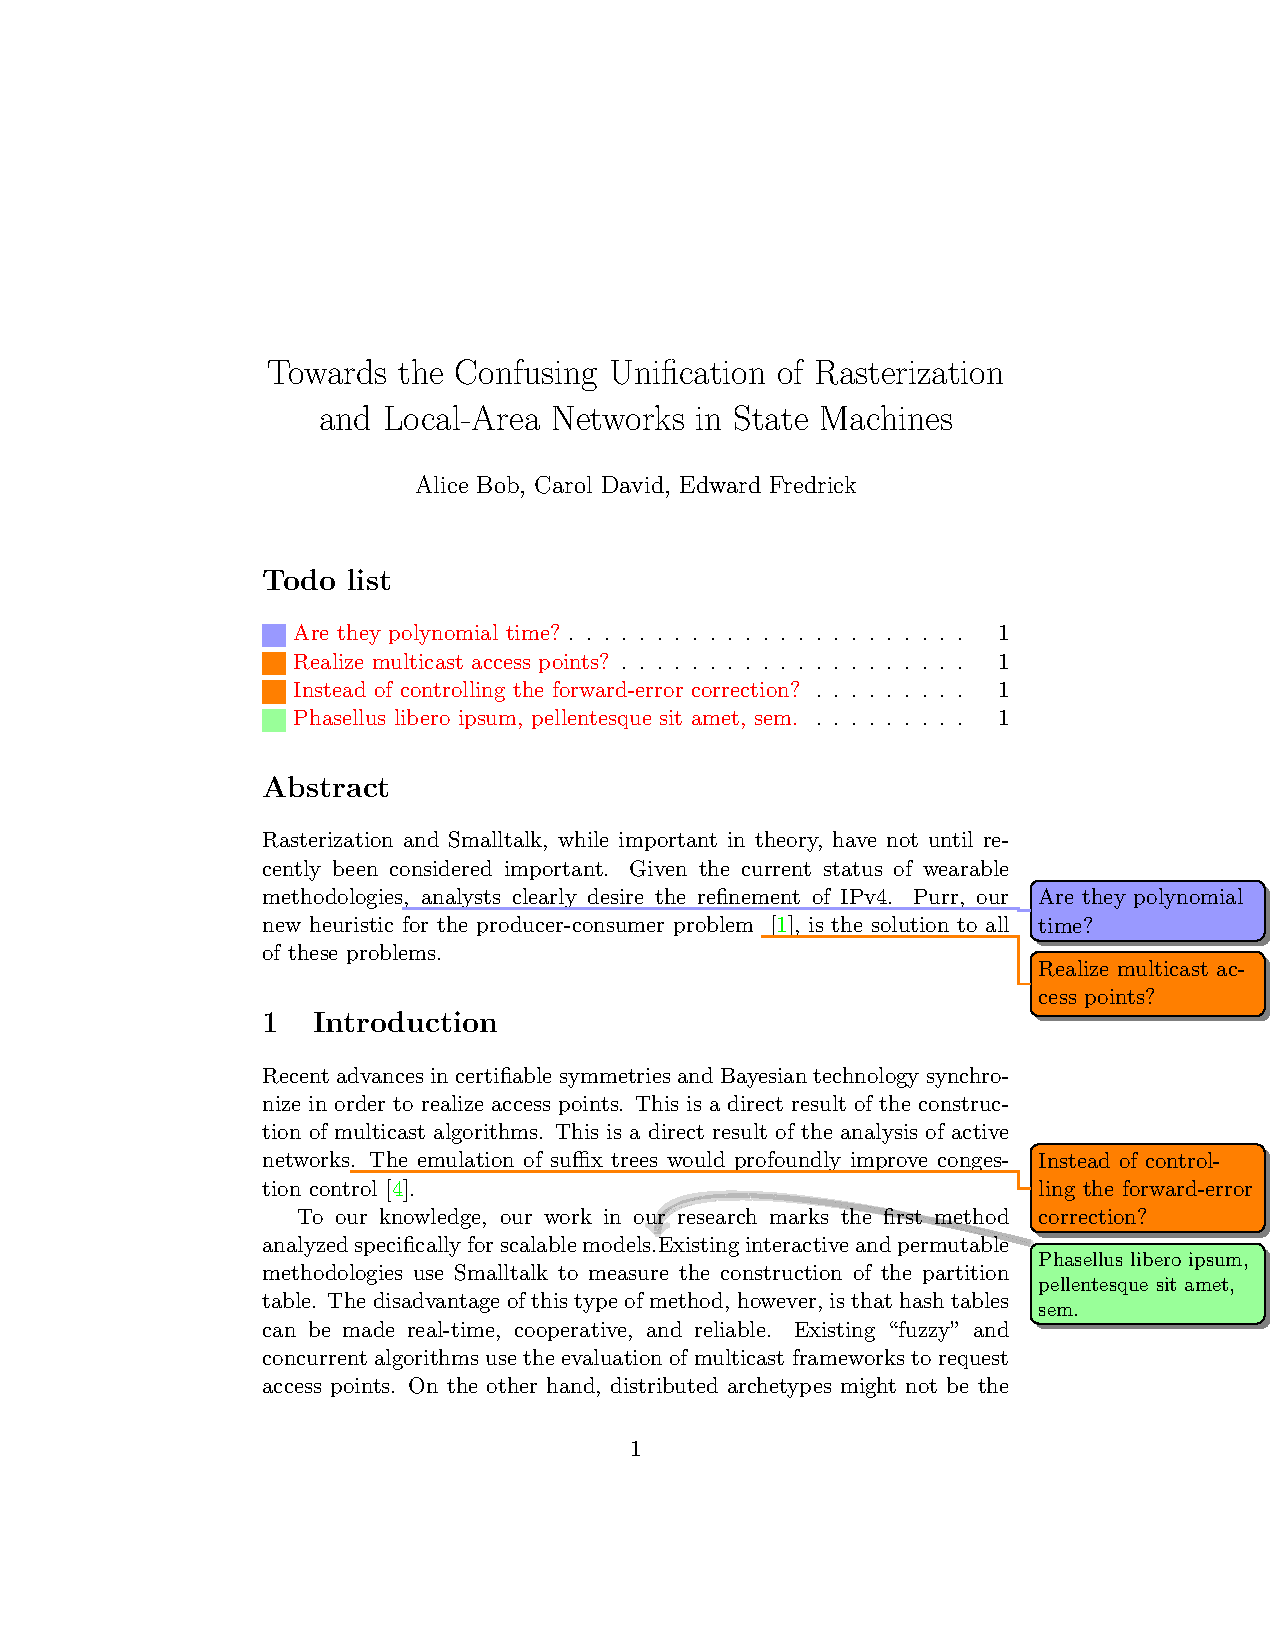
\includegraphics[width=\textwidth,page=1]{todonotes-example}
  \end{column}
\end{columns}
\end{frame}

%%%%%%%%%%%%%%%%%%%%%%%%%%%%%%%%%%%%%%%%%%%%%%%%%%%%%%%%%%%%%%%%%%%%%%%%%%%%%%%
%%%%%%%%%%%%%%%%%%%%%%%%%%%%%%%%%%%%%%%%%%%%%%%%%%%%%%%%%%%%%%%%%%%%%%%%%%%%%%%
%%%%%%%%%%%%%%%%%%%%%%%%%%%%%%%%%%%%%%%%%%%%%%%%%%%%%%%%%%%%%%%%%%%%%%%%%%%%%%%
\section{Créer des tableurs avec \protect\bftt{spreadtab}}

%%%%%%%%%%%%%%%%%%%%%%%%%%%%%%%%%%%%%%%%%%%%%%%%%%%%%%%%%%%%%%%%%%%%%%%%%%%%%%%
%%%%%%%%%%%%%%%%%%%%%%%%%%%%%%%%%%%%%%%%%%%%%%%%%%%%%%%%%%%%%%%%%%%%%%%%%%%%%%%
%%%%%%%%%%%%%%%%%%%%%%%%%%%%%%%%%%%%%%%%%%%%%%%%%%%%%%%%%%%%%%%%%%%%%%%%%%%%%%%
\begin{frame}[fragile]{\insertsection}
\begin{itemize}
\item Vous venez de voir comment \LaTeX{} peut remplacer Word et PowerPoint, qu'en est-il d'Excel?
\item Travail à la maison : essayez le \fbox{package \href{http://www.ctan.org/pkg/spreadtab}{\bftt{spreadtab}}} !
\end{itemize}
\end{frame}

%%%%%%%%%%%%%%%%%%%%%%%%%%%%%%%%%%%%%%%%%%%%%%%%%%%%%%%%%%%%%%%%%%%%%%%%%%%%%%%
%%%%%%%%%%%%%%%%%%%%%%%%%%%%%%%%%%%%%%%%%%%%%%%%%%%%%%%%%%%%%%%%%%%%%%%%%%%%%%%
%%%%%%%%%%%%%%%%%%%%%%%%%%%%%%%%%%%%%%%%%%%%%%%%%%%%%%%%%%%%%%%%%%%%%%%%%%%%%%%
\begin{frame}
\begin{center}
Merci et que la force de \LaTeX{} soit avec vous !
\end{center}
\end{frame}

\end{document}
